% based on a template made by the university of cologne
% http://www.mi.uni-koeln.de/wp-MIEDV/wp-content/uploads/2016/07/LaTeX-Vorlage.zip - 2023-11-02
\documentclass[12pt,a4paper]{scrartcl}

\addtokomafont{sectioning}{\rmfamily}
\usepackage[ngerman]{babel}% deutsches Sprachpaket wird geladen
\usepackage[T1]{fontenc} % westeuropäische Codierung wird verlangt
\usepackage[utf8]{inputenc}% Umlaute werden erlaubt
\usepackage[usenames]{color} % Erlaubt die Benutzung der namen im Farbpaket und deren Änderung
\usepackage{amsmath} % Erweiterung für den Mathe-Satz
\usepackage{amssymb} % alle Zeichen aus msam und msmb werden dargestellt
\usepackage{graphicx} % Graphiken und Bilder können eingebunden werden
%\usepackage{multirow} % erlaubt in einer Spalte einer Tabelle die Felder in mehreren Zeilen zusammenzufassen
\usepackage{enumerate} % erlaubt Nummerierungen
\usepackage{xurl} % Dient zur Auszeichnung von URLs; setzt die Adresse in Schreibmaschinenschrift.
\usepackage[center]{caption}  % Bildunterschrift wird zentriert
%\usepackage{subfigure} % mehrere Bilder können in einer fugure-Umgebung verwendet werden
%\usepackage{longtable} % Diese Umgebung ist ähnlich definiert wie die tabular-Umgebung, erlaubt jedoch mehrseitige Tabellen.
%\usepackage{paralist} % Modifikation der bereits bestehenden Listenumgebungen
\usepackage{lmodern}% Für die Schrift
\usepackage[hidelinks]{hyperref} % Links und Verweise werden innerhalb von PDF Dokumenten erzeugt
%\usepackage{wrapfig} % Das Paket ermöglicht es von Schrift umflossene Bilder und Tabellen einzufügen.
\usepackage{latexsym} % LaTeX-Symbole werden geladen
\usepackage{tikz} % Erlaubt es mit tikz zu zeichnen
\usepackage{tabularx} % Erlaubt Tabellen
\usepackage{algorithm} % Erlaubt Pseudocode
\usepackage{color} % Farbpaket wird geladen
%\usepackage{stmaryrd} % St Mary Road Symbole werden geladen
\usepackage{physics}
\usepackage[version=4]{mhchem} % Chemie: \ce & \pu

\numberwithin{equation}{section} % Nummerierungen der Gleichungen, die durch equation erstellt werden, sind gebunden an die section
\newcommand{\HRule}{\rule{\linewidth}{0.7mm}}

\hypersetup{
  pdftitle={B1.4: Photoelektrischer Effekt},
  pdfcreator={\LaTeX}
}

\setcounter{secnumdepth}{6}
\setcounter{tocdepth}{6}

\begin{document}
\begin{titlepage}
	\pagestyle{empty}

	\begin{center}

	\textsc{\LARGE Universität zu Köln }\\ [0.4cm]
	\textsc{Mathematisch--Naturwissenschaftliche Fakultät} \\[1.5cm]

	
\includegraphics[width=0.45\textwidth]{../media/uni.jpg} \\[1.5cm]  % Uni-Logo wird geladen

	\textsc{\Large Praktikum~B}\\[2mm]
	\textsc{11. Juni 2024}\\[10mm]
	\HRule \\[0.4cm]

		{	\Huge \bfseries B1.4}\\[0.4cm]
			{	\huge \bfseries Photoelektrischer Effekt}\\[0.3cm]
	
	\HRule \\[3cm]

 	\begin{center}
		\textsc{\Large Catherine~Tran } \\[3pt]
		\textsc{\Large Carlo~Kleefisch } \\[3pt]
		\textsc{\Large Oliver~Filla } \\[3pt]
	\end{center}
	\end{center}
\end{titlepage}

\newpage
\tableofcontents
\newpage

\clearpage
\hypertarget{einleitung}{%
\section{Einleitung}\label{einleitung}}

Der photoelektrische Effekt beschreibt die Auslösung von Elektronen aus einem Material, das mit Licht einer bestimmten Frequenz bestrahlt wird. Diese Elektronen haben nach dem Austritt eine kinetische Energie, die von der Frequenz des Lichts abhängt.

Die Energie der Elektronen hängt jedoch nicht von der Intensität des Lichtes ab. Dadurch kann nicht jede elektromagnetische Strahlung für den Photoeffekt verwendet werden. Die Intensität bestimmt stattdessen die Anzahl der Elektronen, die in einer bestimmten Zeit ausgelöst werden und einen Photostrom bilden.

Dieses Phänomen war bereits im 19. Jahrhundert beobachtet worden, konnte jedoch nicht erklärt werden. Ohne die Quantenphysik nahm man an, dass die Energie des Lichts von seiner Amplitude und Intensität abhänge, ähnlich wie bei makroskopischen Wellen. Dies stand jedoch im Widerspruch zum beobachteten Photoeffekt.

\textsc{Albert Einstein} erklärte diesen Effekt im Jahr 1905 durch seine Lichtquantenhypothese. Nach dieser besteht das Licht einer Frequenz $\nu$ aus Quanten mit der Energie $h\nu$. Damit ist der fehlende Zusammenhang von Lichtintensität und kinetischer Energie der Elektronen erklärbar.

\clearpage
\hypertarget{theoretische-grundlagen}{\section{Theoretische Grundlagen}\label{theoretische-grundlagen}}

\subsection{Physikalische Grundlagen}
\subsubsection{Elektrische Felder}
\label{Elektrische Felder}

Das elektrische Feld ist ein Vektorfeld, welches jedem Punkt im Raum den Vektor der elektrischen Feldstärke $\vec{E}$ zuordnet. Diese beschreibt die Coulomb-Kraft $\vec{F}_C$, die auf eine Ladung $Q$ an diesem Ort wirkt.

\begin{eqnarray}
	\vec{E} &=& \frac{\vec{F}_C}{Q}
\end{eqnarray}

\noindent
Feldlinien werden als Darstellungsmittel verwendet und liegen tangential an der Feldstärke $\vec{E}$. Feldlinien beginnen in positiven und enden in negativen Ladungen.

\subsubsection{Spannung}
\label{Spannung}
Um eine elektrische Ladung von einem Ort $A$ zu einem Ort $B$ zu bewegen, muss elektrische Arbeit $W_{AB}$ aufgebracht werden. Sie hängt von der Feldstärke ab.

Die \emph{elektrische Spannung} beschreibt diese Arbeit unabhängig von der zu verschiebenden Ladung $Q$. \cite{Gerthsen}

\begin{eqnarray}
	U_{AB} &=& \frac{W_{AB}}{Q}
\end{eqnarray}

\subsubsection{Transmission von Licht}
Wie jede Welle kann auch Licht ein Medium durchdringen. Der \emph{Transmissionsgrad} $T$ eines Mediums beschreibt, welcher Anteil von einfallender Strahlung transmittiert wird. Er ist der Quotient aus der Beleuchtungsstärke vor dem Medium $I_0$ sowie hinter demselben $I$. \cite{Gerthsen}

\begin{eqnarray}
	T &=& \frac{I}{I_0}
\end{eqnarray}

\noindent
Der Transmissionsgrad eines Mediums hängt im Allgemeinen von der betrachteten Wellenlänge ab. Es gibt verschiedene Filter, um die Strahlungsintensität zu reduzieren.

Ein \emph{Farbfilter} lässt nur Licht einer bestimmten Wellenlänge hindurch. Für diese Wellenlänge beträgt der Transmissionsgrad näherungsweise $1$, für alle anderen Wellenlängen $0$. % Quelle: https://de.wikipedia.org/wiki/Farbfilter

Im Unterschied dazu lässt ein \emph{Graufilter} oder Neutraldichtefilter alle Wellenlängen in gleicher Stärke hindurch. Der Transmissionsgrad ist damit idealerweise unabhängig von der Wellenlänge. % Quelle: https://de.wikipedia.org/wiki/Neutraldichtefilter

\subsubsection{Austrittsarbeit}
Die Austrittsarbeit $W_A$ ist die Energiedifferenz zwischen Fermi--Niveau $E_F$ in einem Material und dem Vakuumniveau mit $E_\mathrm{pot}(\infty)=0$, das dem elektrischen Potential in unendlicher Entfernung entspricht. Da die Fermi--Niveaus materialabhängig sind, trifft dies auch auf die Austrittsarbeit zu. \cite{Demtröder}

\begin{eqnarray}
	W_A &=& E_\mathrm{pot}(\infty) - E_F \\
	W_A &=& -E_F
\end{eqnarray}

\noindent
Das einfachste quantenmechanische Erklärungsmodell ist der Potentialkasten, der in Abbildung \ref{fig:Austrittsarbeit} dargestellt ist.

\begin{figure}[h!]
	\centering
	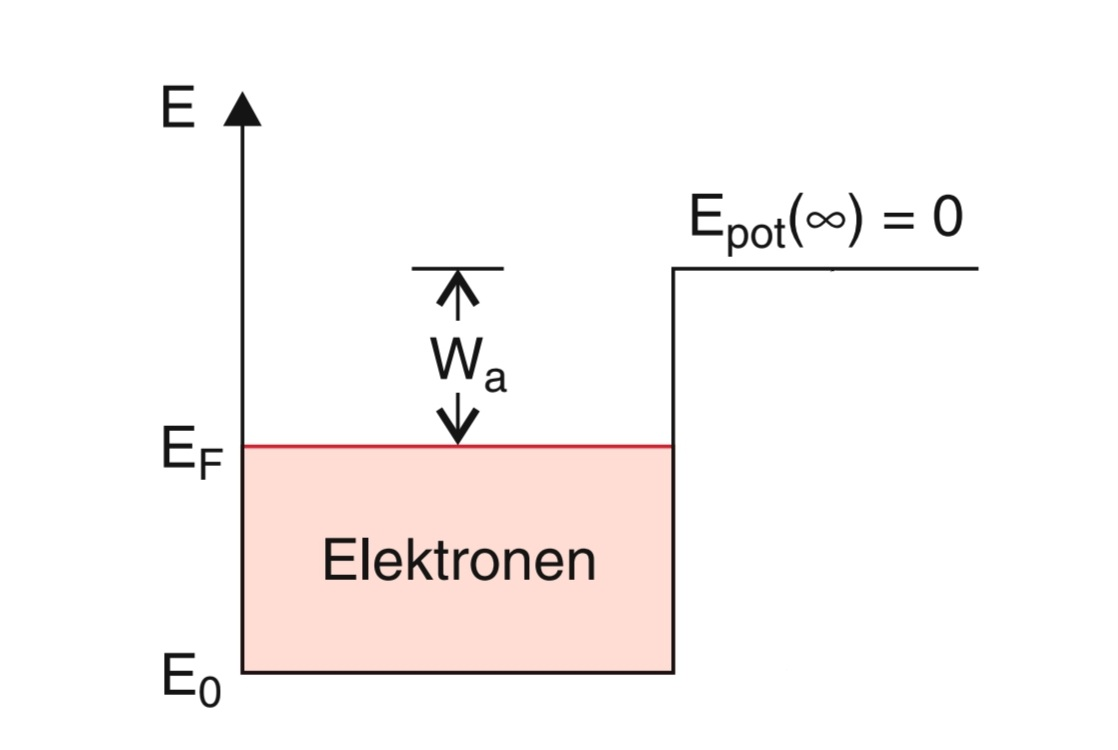
\includegraphics[width=0.5\textwidth]{../media/B1.4/Austrittsarbeit_Potentialkasten.jpg}
	\caption{Austrittsarbeit $W_a$ aus einem Potentialkasten \cite{Demtröder}}
	\label{fig:Austrittsarbeit}
\end{figure}

\subsubsection{Kontaktspannung}
Berühren sich zwei unterschiedliche Metalle mit verschiedenen Austrittsarbeiten, so entsteht eine Spannung an der Kontaktstelle.

Diese \emph{Kontaktspannung} $U_K$ wird durch Elektronen verursacht, die von dem Metall mit der geringeren Austrittsarbeit $W_1$ in das mit der höheren Austrittsarbeit $W_2$ übergehen. Dadurch kommt es zu einem Ladungsungleichgewicht. Dieser Prozess endet in einem Gleichgewichtszustand, wenn $U_K$ der Differenz der Fermi--Niveaus $\Delta E_F$ entspricht.

\begin{eqnarray}
	\Delta E_F &=& e \cdot (\Phi _2 - \Phi _1) \\
		&=& e \cdot U_K \\
	\Delta E_F &=& W_2 - W_1 \\
	\Rightarrow U_K &=& \frac{W_2 -W_1}{e}
\end{eqnarray}

\noindent
Betrachtet man die Elektronen im Metall als Elektronengas, dann gilt die Boltzmann--Verteilung. Die Kontaktspannung lässt sich aus dem Verhältnis der Elektronenzahldichten $n_1$ und $n_2$ bestimmen. Dabei finden die Boltzmann-Konstante $k_B$, die Temperatur $T$ in Kelvin und die Elementarladung $e$ Verwendung.

\begin{eqnarray}
	U_K &=& \frac{k_B T}{e} \ln \left( \frac{n_2}{n_1} \right) \label{eq:Kontaktspannung}
\end{eqnarray}

\noindent
Aufgrund der dichten Gase muss korrekterweise die Fermi--Verteilung verwendet werden. \cite{Gerthsen} Dies wird jedoch in diesem Versuch vernachlässigt.

\subsubsection{Photoeffekt}
Der \emph{äußere photoelektrische Effekt} beschreibt das Auslösen von Elektronen aus einer Materialoberfläche unter Bestrahlung mit elektromagnetischen Wellen. Dazu muss die Strahlung eine Grenzfrequenz $\nu_g$ aufweisen, deren Energie der Austrittsarbeit entspricht.

Ein Lichtquant mit einer Frequenz $\nu$ besitzt eine Energie $h\nu$, die durch das Planck'sche Wirkungsquantum $h$ beschrieben wird. Aufgrund der Energieerhaltung erhält jedes herausgelöste Elektron eine maximale kinetische Energie $E_\mathrm{max}$.

\begin{eqnarray}
	E_\mathrm{max} &=& h\nu - W_A \\
		&=& \frac{1}{2} m_e v^2 \\
	h &=& 4.135 \cdot 10^{-15} \mathrm{\,eV \cdot s}
\end{eqnarray}

\noindent
Die Grenzfrequenz $\nu_g$ kann durch die Austrittsarbeit $W_A$ bestimmt werden.

\begin{eqnarray}
	\nu_g &=& \frac{W_A}{h}
\end{eqnarray}

\noindent
Der Photoeffekt hängt vollständig von der Frequenz ab, nicht von der Intensität der Strahlung. Bei hoher Intensität werden in einem Zeitrahmen mehr Elektronen herausgelöst. Beträgt die Frequenz weniger als die Grenzfrequenz, findet unabhängig von der Intensität kein äußerer Photoeffekt statt.

Die Austrittsarbeit liegt in der Größenordnung Elektronenvolt, beispielsweise $2.1\mathrm{\,eV}$ (Barium) oder $4.91\mathrm{\,eV}$ (Nickel). \cite{Demtröder} Daher kann Licht im sichtbaren und ultravioletten Spektrum den äußeren Photoeffekt auslösen.

Im \emph{inneren Photoeffekt} werden Elektronen nicht aus dem Material gelöst, sondern aus dem Valenzband in das Leitungsband angeregt. Dieser Prozess kann in Halbleitermaterialien stattfinden.

\subsection{Elektrotechnik}
\subsubsection{Funktionsweise einer Photozelle}
Eine Photozelle besteht aus einer Photokathode und einer Anode in einem Glaskolben, siehe Abbildung \ref{fig:photozelle}.

Fällt Licht auf die Photokathode, so werden durch den Photoeffekt Elektronen aus der Kathode gelöst. Einige dieser sogenannten \textit{Photoelektronen} treffen auf die Anode. Dadurch entsteht ein elektrisches Feld zwischen den Elektroden.

\begin{figure}[h]
	\centering
	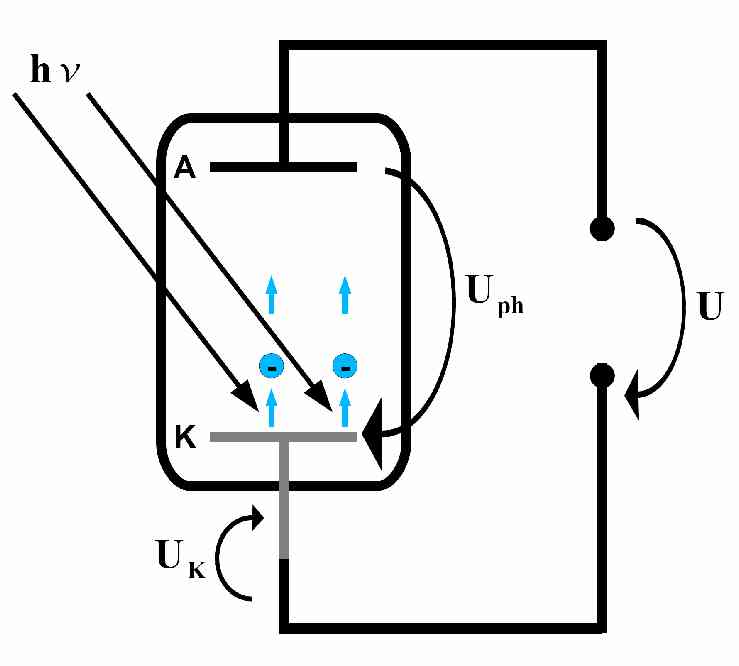
\includegraphics[width=0.4\textwidth]{../media/B1.4/Photozelle.jpg}
	\caption{Darstellung einer Photozelle mit Kathode $K$ und Anode $A$ \cite{uni}}
	\label{fig:photozelle}
\end{figure}

Die Photoelektronen können auf ihrem Weg zur Anode abgebremst werden, indem eine externe Spannung an den Elektroden angelegt wird. Hierbei muss an der Anode eine negative Spannung angelegt werden.

Die \textit{Stoppspannung} $U_{\mathrm{Ph}, 0}$ ist die minimale Spannung, die alle Photoelektronen abbremst. Sie hängt von der Energie des Lichts $h\nu$ mit Frequenz $\nu$ und der Austrittsarbeit $W_A(K)$ der Kathode ab. \cite{Gerthsen}

\begin{eqnarray}
	e \cdot U_{\mathrm{Ph}, 0} &=& h \cdot \nu - W_A (K)
\end{eqnarray}

\subsubsection{stromfreie Spannungsmessung}
Bei stromfreier Spannungsmessung wird die Spannung gemessen, ohne dass Strom durch das Messgerät fließt. Sie wird mittels eines Elektrometers durchgeführt.

Es gibt verschiedene Arten von Elektrometern, die alle nach dem gleichen Prinzip funktionieren. Eine elektrische Ladung ist an einer Art Zeiger angebracht, der sich in einem Kondensator befindet. Wird eine Spannung an den Kondensator angelegt, wird der Zeiger aufgrund des entstehenden elektrischen Feldes ausgelenkt. Eine passend angebrachte Skala ermöglicht die Bestimmung der Spannung anhand der Auslenkung des Zeigers \cite{Gerthsen}.

Eine solche stromfreie Spannungsmessung wird in diesem Versuch verwendet.

\subsubsection{Kontaktspannung}

\clearpage
\hypertarget{durchfuxfchrung}{\section{Durchführung}\label{durchfuxfchrung}}
Eine Photozelle bildet das zentrale Element des Versuchs. Sie wird an einem Messverstärker angeschlossen, der das Signal verstärkt und zum Voltmeter leitet. Als Strahlungsquelle dient eine Quecksilberdampflampe, die nach $10\mathrm{\,min}$ ihre Betriebstemperatur erreicht hat.

Zunächst wird die Energie der Elektronen mit zwei verschiedenen Methoden gemessen, um $\frac{h}{e}$ zu bestimmen. Daraufhin wird die Abhängigkeit des Photostroms von der einfallenden Intensität untersucht. Schließlich werden Leuchtdioden als Strahlungsquellen verwendet, um deren Wellenlängen zu bestimmen.

Am Messverstärker können die Verstärkung und eine Zeitkonstante eingestellt werden. Letztere glättet die Messwerte, indem die Werte über die eingestellte Zeit gemittelt werden. Nach jeder Änderung des Versuchsaufbaus muss der Nullpunkt des Messverstärkers korrekt justiert werden.

\subsection{Energiemessung}
\label{durchführung:Energiemessung}
Es gibt zwei verschiedene Methoden, die Energie der herausgelösten Elektronen zu messen. Entweder wird die Stoppspannung oder die Spannung an der Photozelle gemessen. Ersteres bezeichnet man als Gegenspannungsmethode, letzteres als direkte Methode. Beide Methoden werden in den folgenden Abschnitten \ref{durchführung:Gegenspannung} bzw. \ref{durchführung:direkt} beschrieben.

Zur Bestimmung von $\frac{h}{e}$ und zur Vermessung der LEDs gibt $5$ verschiedene Interferenzfilter, die jeweils auf eine andere Wellenlänge aus dem ultravioletten und sichtbaren Spektrum filtern. Da die Wellenlänge proportional zu der Energie des Lichts ist, wird ein linearer Zusammenhang mit der Steigung $\frac{h}{e}$ zwischen Wellenlänge und Spannung gemessen. Die Eigenschaften der Filter sind in Tabelle \ref{tab:Interferenzfilter} dargestellt.

Dabei ist der Messverstärker auf den Modus ``Elektrometer'' eingestellt. Weiterhin wird der Innenwiderstand $10^{13}\,\Omega$ verwendet, um den Photostrom möglichst zu stoppen. Der Messverstärker wird mit $10$--facher Verstärkung und der Zeitkonstante $0.3\mathrm{\,s}$  verwendet.

\begin{table}[h!]
	\centering
	\begin{tabular}{c|c|c}
		Filter & Farbe & $\lambda$ $[\mathrm{nm}]$ \\
		\hline
		$1$ & UV & $366$ \\
		$2$ & Violett & $405$ \\
		$3$ & Blau & $436$ \\
		$4$ & Grün & $546$ \\
		$5$ & Gelb & $578$ \\
	\end{tabular}
	\caption{Eigenschaften der Interferenzfilter mit $\Delta \lambda = \pm 7\mathrm{nm}$}
	\label{tab:Interferenzfilter}
\end{table}

\subsubsection{Gegenspannungsmethode}
\label{durchführung:Gegenspannung}

Bei der Gegenspannungsmethode wird die Stoppspannung gemessen, bei der der Photostrom verschwindet.  Der Schaltplan ist in Abbildung \ref{fig:Schaltplan Gegenspannungsmethode} zu sehen. Anschließend wird das Gegenspannungsmodul an die Photozelle angeschlossen.

Vor jeder Messung muss der Nullpunkt korrekt justiert werden. Dann wird Gegenspannung langsam von $0\mathrm{\,V}$ erhöht, bis der Spannungsabfall am Elektrometer verschwindet. Die angezeigte Gegenspannung ist die Stoppspannung $U_0$.

\begin{figure}[h!]
	\centering
	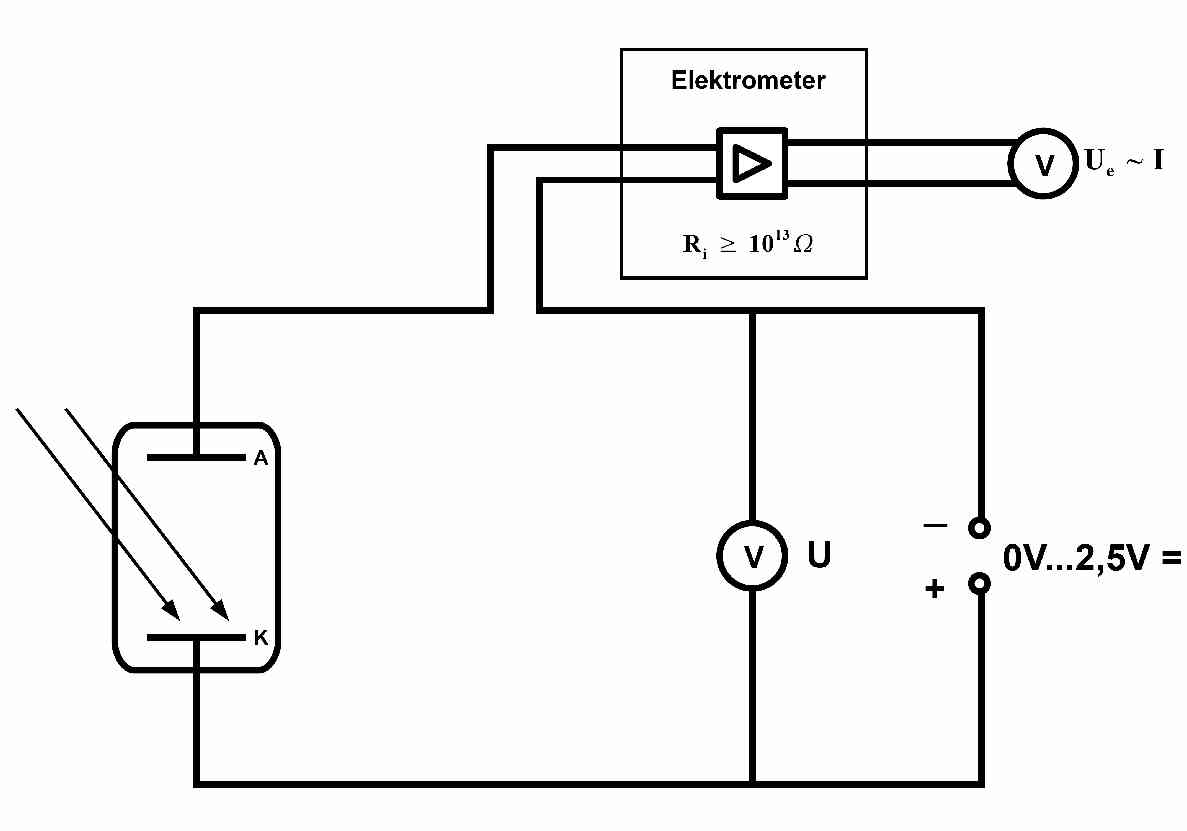
\includegraphics[width=0.7\textwidth]{../media/B1.4/Schaltplan_Gegenspannungsmethode.jpg}
	\caption{Schaltplan der Gegenspannungsmethode}
	\label{fig:Schaltplan Gegenspannungsmethode}
\end{figure}

\subsubsection{direkte Methode}
\label{durchführung:direkt}

Anstatt der Gegenspannung kann auch die Spannung an der Photozelle direkt gemessen werden. Dazu wird die Zelle mit dem Elektrometer verbunden. Wie bei der Gegenspannungsmethode ist der Messverstärker als ``Elektrometer'' eingestellt, der Innenwiederstand beträgt auch hier $10^{13}\,\Omega$.

Anders als bei der Gegenspannungsmethode muss die Photozelle bei der direkten Methode vor jeder Messung entladen werden, um die Spannung zurückzusetzen. Zu diesem Zweck besitzt sie einen Kurzschlussschalter.

\begin{figure}[h!]
	\centering
	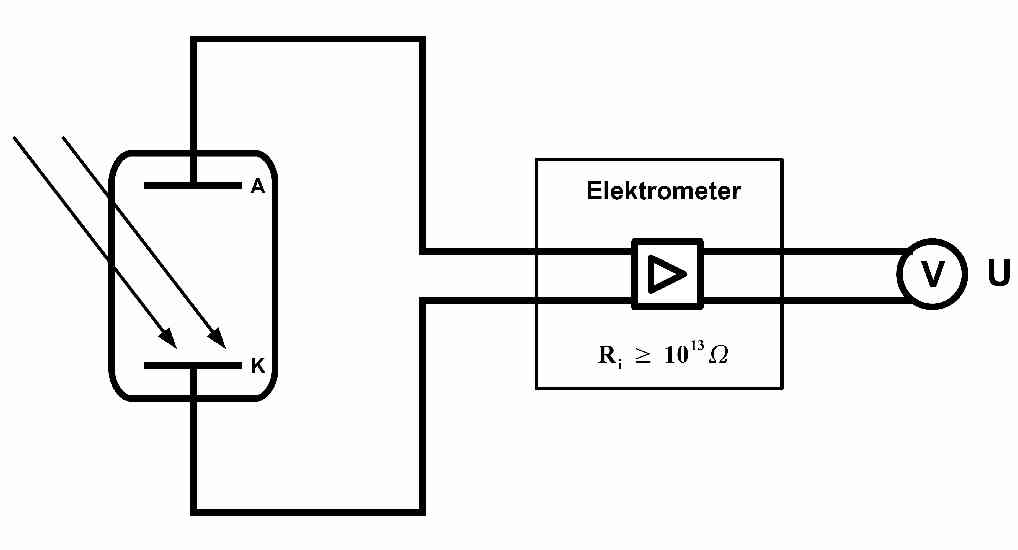
\includegraphics[width=0.7\textwidth]{../media/B1.4/Schaltplan_direkte_Methode.jpg}
	\caption{Schaltplan der direkten Methode}
	\label{fig:Schaltplan direkt}
\end{figure}

\subsection{Photostrom}

Zur Messung des Photostroms wird der Messverstärker auf ``Low Drift''. Der Innenwiderstand wird auf $10\mathrm{\,k\Omega}$ heruntergeregelt, um einen Photostrom zu ermöglichen. Die Messung des Stroms erfolgt indirekt über eine Spannung, dazu wird ein Widerstand $R=10\mathrm{\,k\Omega}$ benutzt.

Die Zeitkonstante wird wie bei den vorherigen Messungen in Abschnitt \ref{durchführung:Energiemessung} als $0.3\mathrm{\,s}$ eingestellt, der Messverstärker dagegen auf $10^4$--fache Verstärkung erhöht. Da der Photostrom schwach ist, muss das Signal deutlich mehr verstärkt werden.

Für diesen Versuchsteil wird die \nameref{durchführung:direkt} verwendet, der Schaltplan ist in Abbildung \ref{fig:Schaltplan Photostrom} zu sehen. Die gemessene Spannung $U_e$ ist durch Ohm'sche Gesetz proportional zu dem Photostrom $I_\mathrm{Ph}$.

\begin{figure}[h!]
	\centering
	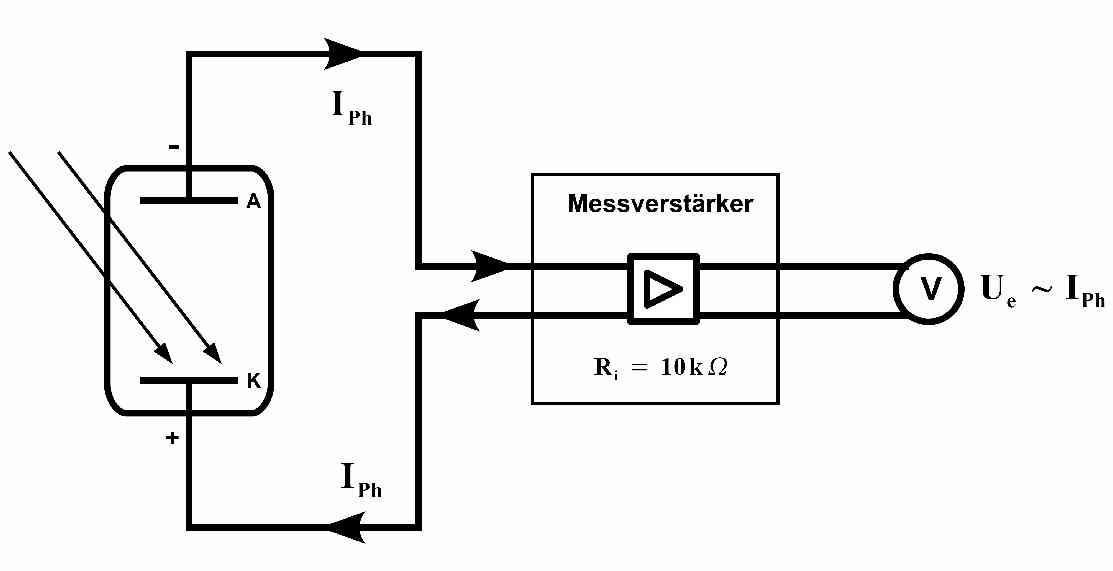
\includegraphics[width=0.7\textwidth]{../media/B1.4/Schaltplan_Photostrom.jpg}
	\caption{Schaltplan der Photostrommessung}
	\label{fig:Schaltplan Photostrom}
\end{figure}

\subsubsection{Photostrom}
Zur Messung des Photostroms werden abwechselnd der blaue und der grüne Interferenzfilter verwendet, zusammen mit einem von $6$ Graufiltern. Die Eigenschaften der Graufilter sind in Tabelle \ref{tab:Graufilter} dargestellt, die der Interferenzfilter in Tabelle \ref{tab:Interferenzfilter} in Abschnitt \ref{durchführung:Energiemessung}. Die Graufilter sind zwischen Interferenzfilter und Photozellengehäuse positioniert.

\begin{table}[h!]
	\centering
	\begin{tabular}{c|c|c|c|c|c|c}
		$\lambda$ $[\mathrm{nm}]$ & \multicolumn{6}{c}{Transmissionsgrad $T$ $[\%]$} \\
		& $1$ & $2$ & $3$ & $4$ & $5$ & $6$ \\
		\hline
		$436$ & $68$ & $48$ & $33$ & $28$ & $20$ & $14$ \\
		$546$ & $67$ & $46$ & $31$ & $23$ & $16$ & $11$
	\end{tabular}
	\caption{Eigenschaften der Graufilter mit $\Delta T=1\,\%$}
	\label{tab:Graufilter}
\end{table}

\subsubsection{Intensität}
Die direkte Messmethode aus Abschnitt \ref{durchführung:direkt} wird zudem dazu verwendet, die Abhängigkeit des Photostroms von der Intensität zu messen. Dabei wird die Stoppspannung mit dem grünen Interferenzfilter je einmal mit und ohne Graufilter $1$ gemessen. Dieser wird vor den Interferenzfilter gehalten, ohne befestigt zu werden.

\subsection{Leuchtdioden}

Zuletzt sollen die Wellenlängen von drei verschiedenen Leuchtdioden bestimmt werden.

Die jeweilige Leuchtdiode wird auf das Photozellengehäuse gesteckt und mit $I=100\mathrm{\,mA}$ betrieben. Dann wurde die Spannung mit der direkten Methode bestimmt, die in Abschnitt \ref{durchführung:direkt} beschrieben ist.

Für die Messungen werden Leuchtdioden mit den Farbbezeichnungen ``blue'', ``verde'' und ``true green'' verwendet. Der Schaltplan ist in Abbildung \ref{fig:Schaltplan LEDs} ersichtlich.

\begin{figure}[h!]
	\centering
	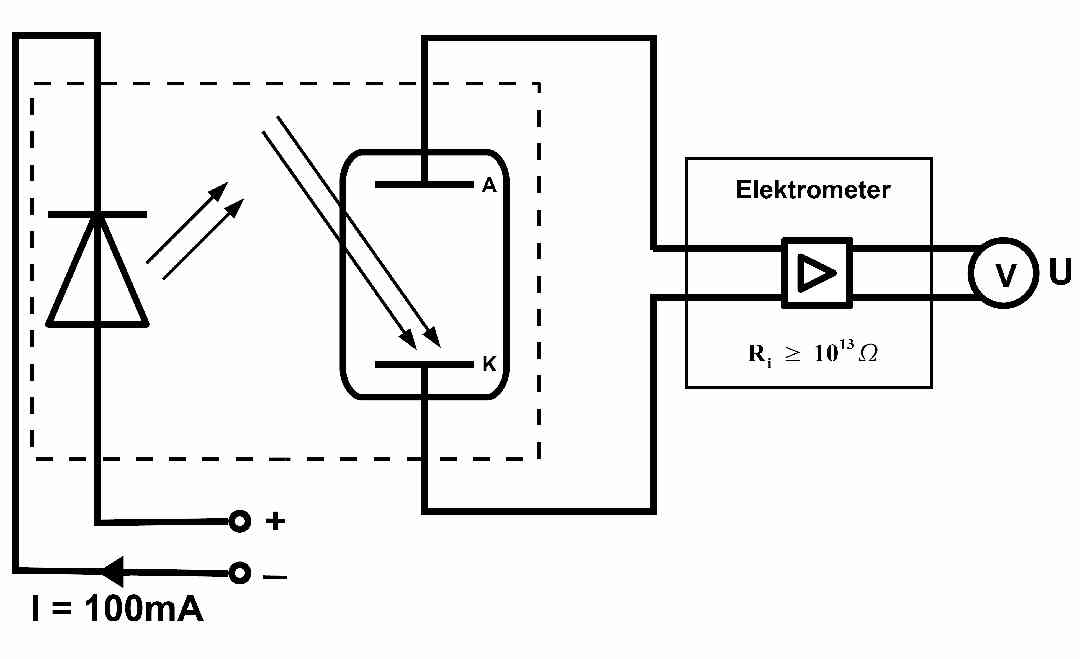
\includegraphics[width=0.7\textwidth]{../media/B1.4/Schaltplan_LED.jpg}
	\caption{Schaltplan der Messungen mit LEDs}
	\label{fig:Schaltplan LEDs}
\end{figure}


\clearpage
\hypertarget{auswertung}{\section{Auswertung}\label{auswertung}}
\subsection{Bestimmung von $h/e$}

\subsubsection{Gegenspannungsmethode}

\begin{table}[h!]
	\centering
	\begin{tabular}{c|c|c}
		Filter & Farbe & $U_0$ $[V]$ \\
		\hline
		$1$ & UV & $1.769$ \\
		$2$ & Violett & $1.434$ \\
		$3$ & Blau & $1.232$ \\
		$4$ & Grün & $0.705$ \\
		$5$ & Gelb & $0.645$ \\
	\end{tabular}
	\caption{Messergebnisse nach der Gegenspannungsmethode mit $\Delta U_0=\pm 1\mathrm{\,mV}$}
	\label{tab:Gegenspannungsmethode}
\end{table}

\subsubsection{direkte Messmethode}
Schon während der Messung fiel die große Ähnlichkeit der Messwerte mit denen aus der vorherigen Messung auf. Dass die Werte eher minimal kleiner sind liegt vermutlich an einem reduzierten Rauschen aus der Umgebung, da die nicht--abgeschirmten Kabel des Aufbaus noch weiter von der Photozelle entfernt waren.

\begin{table}[h!]
	\centering
	\begin{tabular}{c|c|c}
		Filter & Farbe & $U$ $[V]$ \\
		\hline
		$1$ & UV & $1.770$ \\
		$2$ & Violett & $1.434$ \\
		$3$ & Blau & $1.232$ \\
		$4$ & Grün & $0.696$ \\
		$5$ & Gelb & $0.635$ \\
	\end{tabular}
	\caption{Messergebnisse nach der direkten Methode mit $\Delta U_0=\pm 1\mathrm{\,mV}$}
	\label{tab:direkten Methode}
\end{table}

\subsection{Photostrom}
\subsubsection{Photoströme}
Bei der Messung der Photoströme trat ein Nullpunktsfehler von $1\mathrm{\,mV}$ auf. Der Messverstärker wurde auf $10^4$ gestellt, die Zeitkonstante auf $0.3\mathrm{\,s}$. Der Photostrom wurde indirekt über einen Widerstand $R=10\mathrm{\,k\Omega}$ gemessen.

\begin{table}[h!]
	\centering
	\begin{tabular}{c|c|c|c|c|c|c|c|c}
		 	&& \multicolumn{7}{c}{Photostrom $U_\mathrm{Ph}$ $[\mathrm{V}]$} \\
		Filter & Farbe & ohne & $1$ & $2$ & $3$ & $4$ & $5$ & $6$ \\
		\hline
		$3$ & Blau & $1.777$ & $1.486$ & $1.067$ & $0.807$ & $0.655$ & $0.440$ & $0.338$ \\
		$4$ & Grün & $0.608$ & $0.536$ & $0.357$ & $0.265$ & $0.190$ & $0.126$ & $0.090$
	\end{tabular}
	\caption{Messungen der Photoströme über mit $\Delta U_\mathrm{Ph}=1\mathrm{\,mV}$}
	\label{tab:Photostrom}
\end{table}

\subsubsection{Intensität}
Ohne den Graufilter wurde eine Photospannung von $U_0=0.688\pm0.001\mathrm{\,V}$ gemessen, mit Graufilter $6$ eine von $U_0^\prime=0.693\pm0.001\mathrm{\,V}$. Aufgrund dieser Abweichungen sollte der Fehler auf zumindest $\pm 3\mathrm{\,mV}$ erhöht werden.

\subsection{Untersuchung von Leuchtdioden mit der Photozelle}
\begin{table}[h!]
	\centering
	\begin{tabular}{l|c}
		Bezeichnung & $U_0$ $[\mathrm{V}]$ \\
		\hline
		blue & $1.047$ \\
		verde & $0.891$ \\
		true green & $0.807$ \\
	\end{tabular}
	\caption{Messungen der LEDs mit $\Delta U_0=1\mathrm{\,mV}$}
	\label{tab:LEDs}
\end{table}


\clearpage
\hypertarget{fazit}{%
\section{Fazit}\label{fazit}}

\clearpage
\hypertarget{literatur}{%
\section{Literatur}\label{literatur}}
\renewcommand{\section}[2]{}

\begin{thebibliography}{99}
\bibitem{Demtröder}
	W. Demtröder, ``Experimentalphysik 3'', $5.$ Auflage, Springer Verlag,
	DOI~\href{https://doi.org/10.1007/978-3-662-49094-5}{10.1007/978-3-662-49094-5}
\bibitem{Gerthsen}
	D. Meschede, ``Gerthsen Physik'', $25.$ Auflage, Springer Verlag,
	DOI~\href{https://doi.org/10.1007/978-3-662-45977-5}{10.1007/978-3-662-45977-5}
\bibitem{uni}
		Universität zu Köln, ``B1.4: Photoeffekt: Bestimmung von $h/e$'', Juli 2008,
		Online verfügbar unter \url{https://teaching.astro.uni-koeln.de/sites/default/files/praktikum_b/Anleitung_1.4.pdf},
		Abruf am 10.04.2024
\end{thebibliography}
\end{document}
